\documentclass[aspectratio=169,11pt]{beamer}
\usepackage[T1]{fontenc}
\usepackage{lmodern}
\usepackage{amsmath}
\usepackage{graphicx}
\graphicspath{{figures/}}

% ---- OSU look ----
\definecolor{osuorange}{HTML}{DC4405}
\definecolor{osudark}{HTML}{1A1A1A}
\definecolor{osugray}{HTML}{4D4D4D}

\usetheme{default}
\setbeamercolor{title}{fg=osuorange}
\setbeamercolor{frametitle}{fg=white,bg=osuorange}
\setbeamercolor{structure}{fg=osuorange}
\setbeamercolor{normal text}{fg=osudark}
\setbeamercolor{itemize item}{fg=osuorange}
\setbeamercolor{itemize subitem}{fg=osuorange}
\setbeamerfont{frametitle}{series=\bfseries}
\setbeamerfont{title}{series=\bfseries}
\setbeamertemplate{itemize item}{\raisebox{0.25ex}{\small\textcolor{osuorange}{$\blacktriangleright$}}}
\setbeamertemplate{itemize subitem}{\textcolor{osuorange}{\textbullet}}
\setbeamertemplate{navigation symbols}{}
\setbeamertemplate{footline}{%
  \hfill\textcolor{osugray}{\footnotesize\insertframenumber}\hspace{1.2em}\vspace{0.8em}}

% thin orange rule under frame title
\setbeamertemplate{frametitle}{%
  \vspace{0.4em}\hspace{0.2em}\textcolor{osuorange}{\bfseries\insertframetitle}\par
  \vspace{-0.2em}{\color{osuorange}\rule{\linewidth}{1.2pt}}}

\title{\textbf{Recovering the Hidden Digit}}
\subtitle{An electrical tomography inverse problem}
\author{Travis Whitney \quad Cole Seifert \quad Alexander Nutt}
\institute{AI 539, Oregon State University}
\date{Project 1 Competition, Spring 2026}

\begin{document}

\begin{frame}
  \titlepage
\end{frame}

%-------------------------------------------------------------
\begin{frame}{What we are solving}
\begin{columns}[T]
\column{0.58\textwidth}
\vspace{0.5em}
Electrodes around the edge of a box push small currents through it and measure
the resulting voltages. We are handed \textbf{1900 of these readings}.

\vspace{0.6em}
Hidden inside the box is a \textbf{handwritten digit}, drawn as a region that
conducts electricity differently from its surroundings. Our job is to figure
out which digit is inside, using only the readings.

\vspace{0.6em}
Going \textbf{forward} (digit to readings) is a quick physics simulation we
call $F$. We have to go \textbf{backward} (readings to digit), which is the
hard part.

\column{0.42\textwidth}
\centering
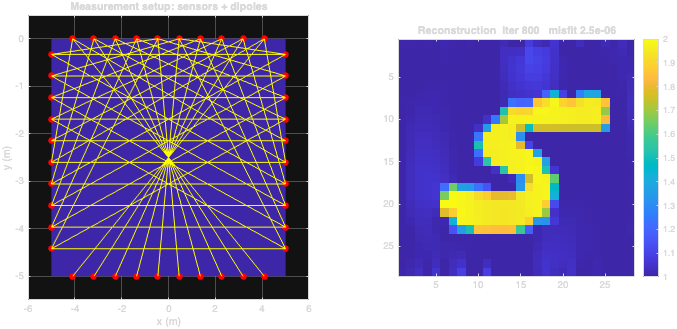
\includegraphics[width=\linewidth]{demo_last.png}\\
{\footnotesize\color{osugray} The sensor setup (left) and a reconstruction we
produced (right).}
\end{columns}
\end{frame}

%-------------------------------------------------------------
\begin{frame}{Why it is hard}
There are two problems, and together they make a direct approach fail.

\vspace{0.8em}
\textbf{1. Many digits give nearly the same readings.}
The edge sensors only pick up a blurred summary of the inside, so very
different digits can produce almost identical readings. Think of a shadow on a
wall: many shapes cast the same shadow, so the shadow alone does not tell you
the shape.

\vspace{0.8em}
\textbf{2. Small measurement errors blow up.}
The readings are slightly noisy, and undoing the blur magnifies that noise a
lot.

\vspace{0.9em}
So ``find any image whose readings match'' gives garbage. We have to tell the
method what a real answer should look like. That piece of knowledge is called
a \textbf{prior}, and choosing it well is the whole game.
\end{frame}

%-------------------------------------------------------------
\begin{frame}{What we tried, and the lesson it taught us}
\begin{columns}[T]
\column{0.54\textwidth}
\vspace{0.3em}
We tried priors from simple to smart:
\begin{itemize}
\item \textbf{Generic rules} (smooth, or mostly blank): only blurry blobs.
\item \textbf{Linear prior from MNIST} (PCA): clean digit shape and the
\emph{lowest} error, but the \textbf{wrong digit}.
\item \textbf{Nonlinear prior} (small neural net): the \textbf{correct digit}.
\end{itemize}

\vspace{0.6em}
The surprise: the lowest-error method gave the wrong answer. Matching the
readings better than the noise allows just fits noise.

\vspace{0.4em}
\textbf{\textcolor{osuorange}{The prior matters, not the error.}}

\column{0.46\textwidth}
\centering
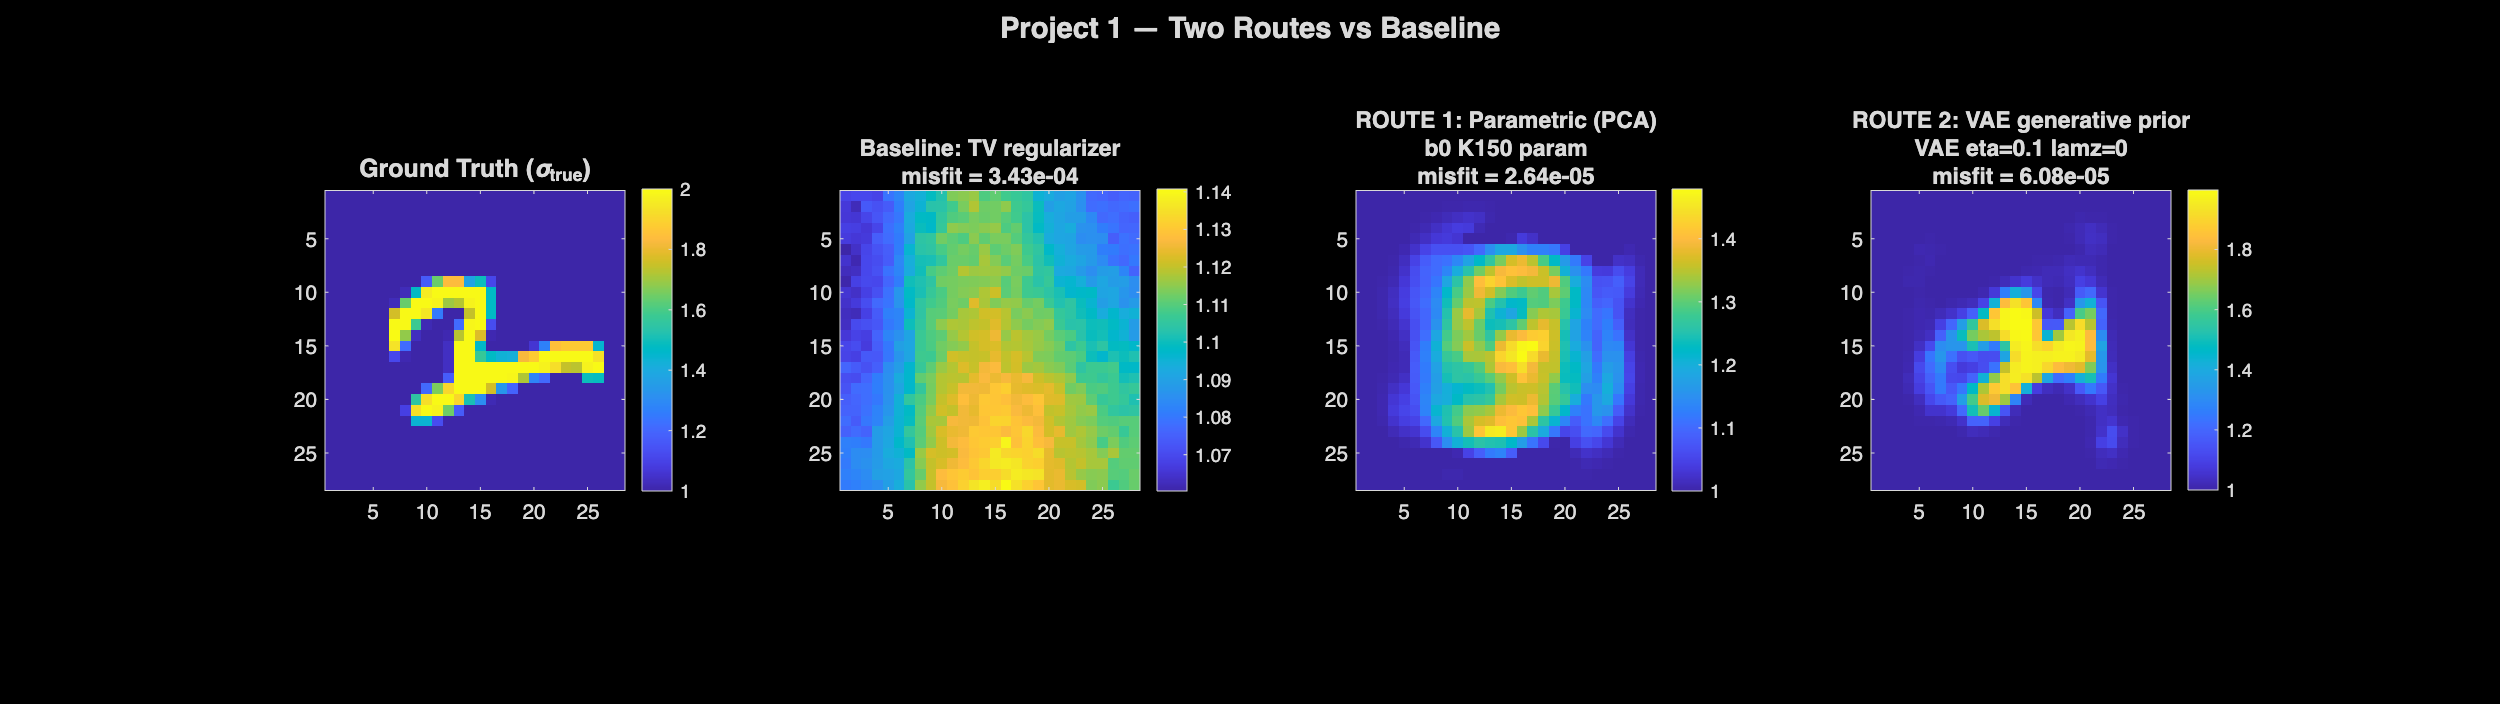
\includegraphics[width=\linewidth]{two_route_comparison.png}\\
{\footnotesize\color{osugray} True digit, then three methods. The
lowest-error result (third panel) is the wrong digit.}
\end{columns}
\end{frame}

%-------------------------------------------------------------
\begin{frame}{The real obstacle: many answers fit}
\begin{columns}[T]
\column{0.52\textwidth}
\vspace{0.6em}
Because several digits each fit the readings reasonably well, the landscape of
possible answers has \textbf{many separate low points}, one near each plausible
digit.

\vspace{0.6em}
A method that just walks downhill settles into whichever low point it starts
nearest, and stops there. We checked this directly: start the search at a 2 and
it returns a 2; start it at a 5 and it returns a 5. The readings alone do not
choose the digit.

\vspace{0.6em}
The fix is a search that looks at \textbf{all} the options at once, instead of
rolling into the nearest one.

\column{0.48\textwidth}
\centering
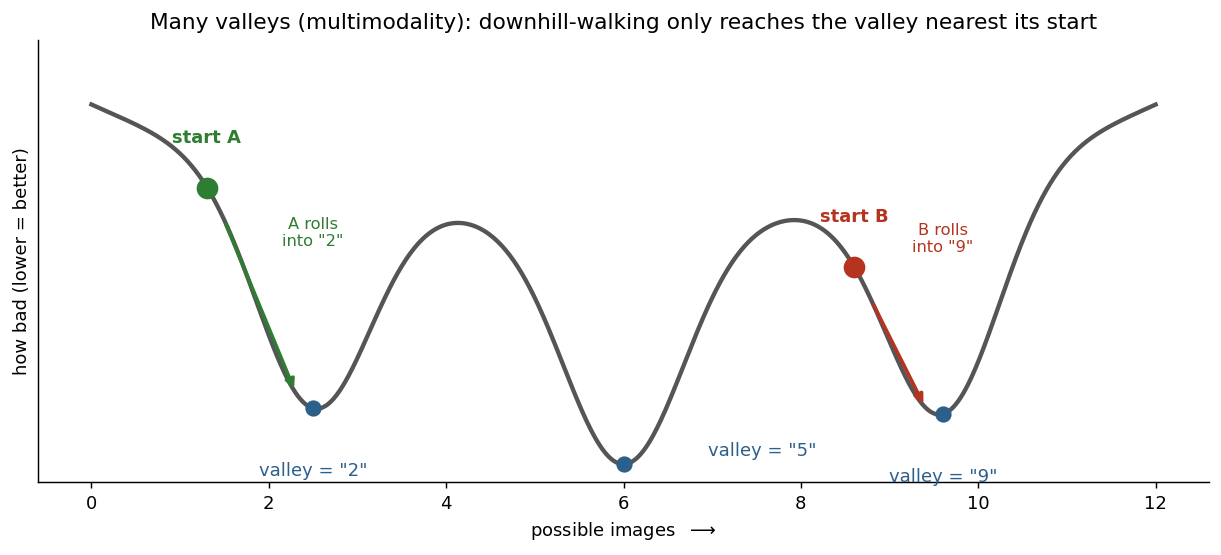
\includegraphics[width=\linewidth]{fig_valleys.png}\\
{\footnotesize\color{osugray} Downhill search reaches only the nearest
``valley,'' so it can lock onto the wrong digit.}
\end{columns}
\end{frame}

%-------------------------------------------------------------
\begin{frame}{Our method}
\textbf{The insight.} The project says the hidden image is essentially one of
the MNIST digits, and we have all 60{,}000. So we check them all instead of
searching blindly.

\vspace{0.5em}
\textbf{Stage 1, identify.} For each of the 60{,}000 real digits, simulate its
readings with $F$ and compare to the measured ones. Keep the closest. Checking
every option means we cannot lock onto the wrong digit.

\vspace{0.5em}
\textbf{Stage 2, polish.} From that best match, take a few downhill steps to
sharpen the exact shape. Safe now, since Stage 1 found the right digit.

\vspace{0.2em}
\centering
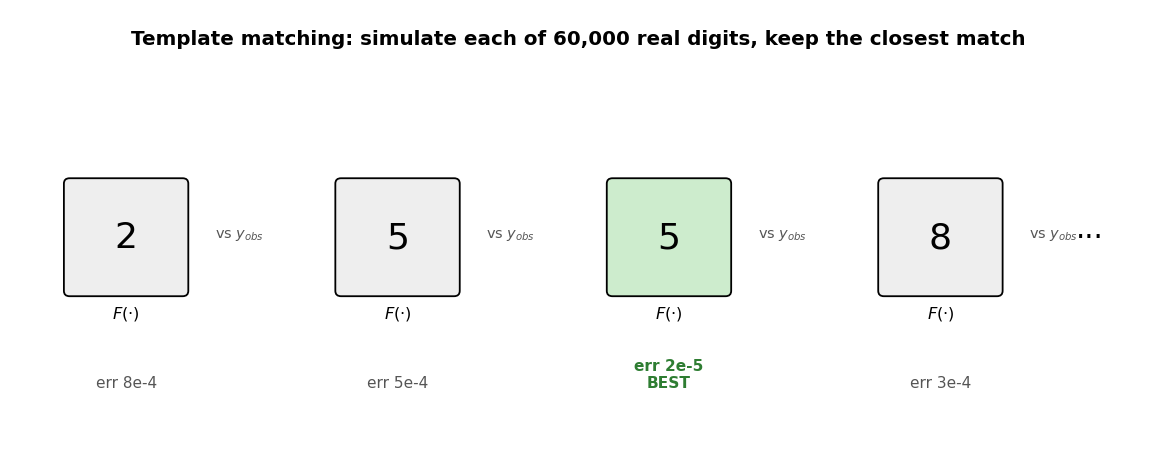
\includegraphics[width=0.62\linewidth]{fig_template_match.png}
\end{frame}

%-------------------------------------------------------------
\begin{frame}{What we recovered}
\begin{columns}[T]
\column{0.5\textwidth}
\centering
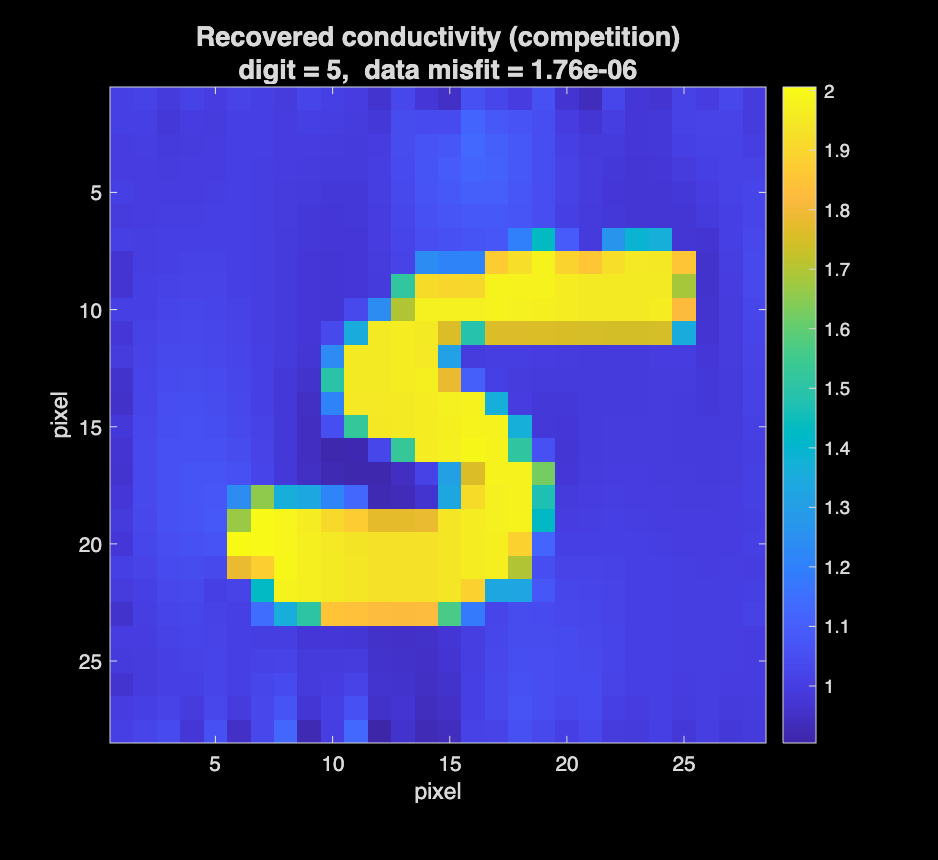
\includegraphics[width=\linewidth]{competition_answer.png}
\column{0.5\textwidth}
\vspace{1.2em}
From the competition data, the hidden digit is a \textbf{5}.

\vspace{0.7em}
The eight best matches were almost all the same 5, so we are confident in the
identity.

\vspace{0.7em}
After polishing, the reconstruction matches the readings about \textbf{200
times better} than the starter method, and the picture is clean and sharp.
\end{columns}
\end{frame}

%-------------------------------------------------------------
\begin{frame}{Summary}
\begin{itemize}
\item The problem is hard because many digits fit the readings and noise blows
up, so matching the readings is not enough.
\item Across everything we tried, the prior mattered more than the error. The
lowest-error method actually returned the wrong digit.
\item Our method uses the strongest prior available, the real digits
themselves, and a search that checks every one, so it never gets trapped on
the wrong digit. Then it polishes the winner.
\item \textbf{Result: a clean 5}, recovered far more accurately than the
baseline.
\end{itemize}

\vspace{1.0em}
\begin{center}
{\large\textcolor{osuorange}{\textbf{Thank you. Questions?}}}
\end{center}
\end{frame}

%-------------------------------------------------------------
\begin{frame}{Backup: does the method generalize?}
\centering

\includegraphics[width=0.96\linewidth]{validation_0to9.png}

\vspace{0.5em}
\raggedright
\footnotesize
Same method, ten \textbf{unseen} test digits (one of each, none in our
dictionary): \textbf{9 of 10 recovered correctly}. Rows are the true digit, the
Stage 1 match (green means correct class), and the refined result. The one miss
is an unseen 5 read as a 6, and it was the least confident case: that handwritten
5 has a looped bottom that resembles a 6. On the competition data the top eight
matches were almost all 5's, so that identity is not a close call.
\end{frame}

\end{document}
